% To teach: curation, presentation, feedback

% test account: labsmbatest, wharton1
% See {\it Notebook} 2008-6-4 pages 6--7,  2008-7-15 pages 38--40 and {\it Daybook}2008-8-14, pages 47--8.
% On the cosine measure of similarity:
% http://www.miislita.com/information-retrieval-tutorial/cosine-similarity-tutorial.html


% Citation: "The outbreak of cooperation among success-driven
% individuals under noisy conditions." By Dirk Helbing and Wenjian
% Yu. Proceedings of the National Academy of Sciences, Vol. 106, No. 8,
% Feb. 23, 2009.

% \begin{figure}[htbp] %  figure placement: here, top, bottom, or page
%    \centering
%    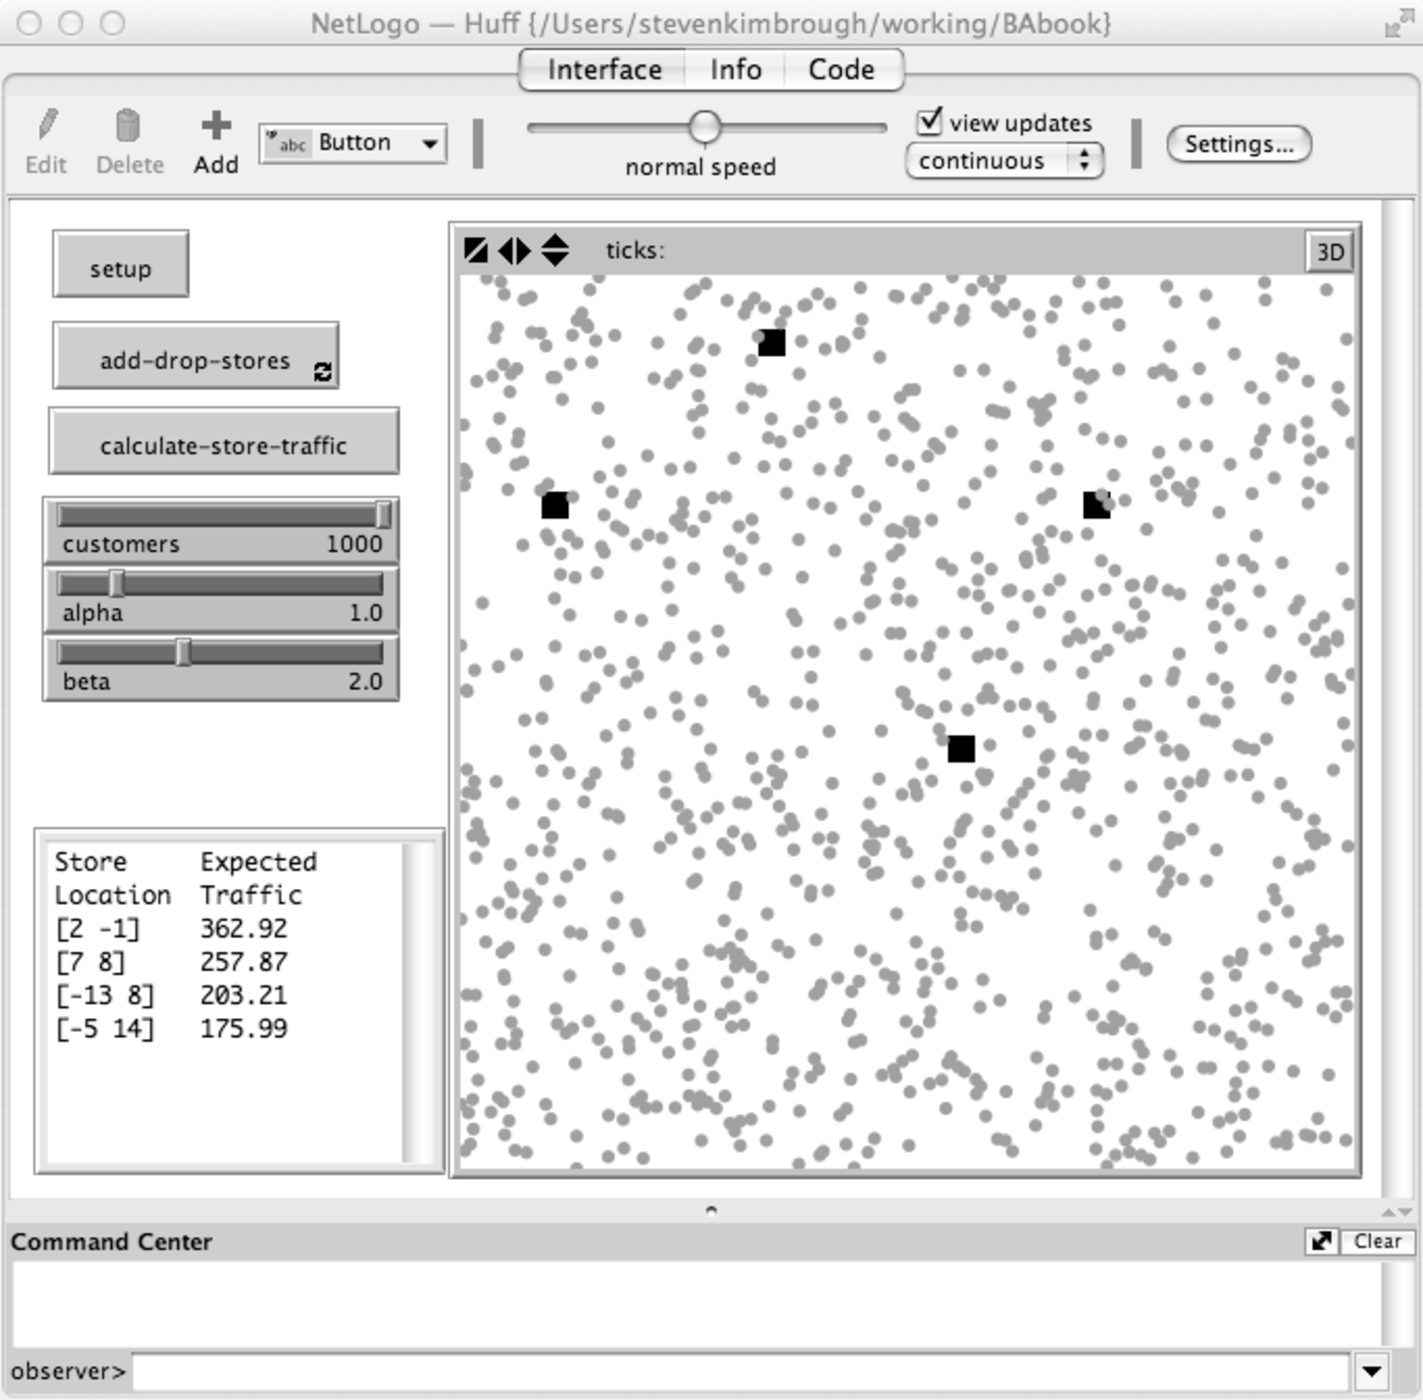
\includegraphics[width=\textwidth]{figures/HuffPatches.pdf}  
%    \caption{Huff, a NetLogo implementation of Huff's model.} % using random-seed 22478
%    \label{fig:huffnlogo}
% \end{figure}

\def\noop#1{}
\def\mlb{MATLAB}
\def\figtop{\rule{\textwidth}{0.5mm}}
\def\figbot{\rule{\textwidth}{0.5mm}}
%%%%%%%%%%%%%%%%%%%%%%%%%
   



 \def\year{2016}
 \def\lastclass{Wednesday, April 29, \year}
%  \def\matlabcasedue{9 p.m. on Monday, March 30, 2015}
%  \def\groupassignmentdue{5 p.m. on Tuesday, May 5, 2015}
%  \def\pythoncasedue{5 p.m. on Thursday, May 7, 2015}
% \def\nis{../../../books/RobustDecisionMaking/NewImages/}
% \def\mlb{MATLAB}
% \def\mb{{\it DAMbook}}
\def\noop#1{}
\def\place{TBA}
\def\figtop{\rule{\textwidth}{0.5mm}}
\def\figbot{\rule{\textwidth}{0.5mm}}
\noop{
\section{Readings}
\section{Lecture notes}
\section{Exercises}
\section{In class assignments}
\section{Case assignments}
  }
 
  
\newtheorem{exercise}{Exercise}
\documentclass[11pt]{book}
\makeindex
\usepackage{url}
\usepackage{palatino}
%
\usepackage{hyperref}
\usepackage{color}
\usepackage{amssymb}

\usepackage{makeidx}
%\usepackage{geometry}
%\geometry{textwidth=6.5in}

\usepackage{rotating} % for sideways and sidewaystable, etc. environments
% the following package, when present, lets the figures and tables orient oppositely on even and odd pages
\usepackage{lscape} 
\usepackage{natbib}

%%%%%% From KAPSARC document, for funny characters
\usepackage{etoolbox}
\usepackage{pifont}
%%%%%%%%%%%%%%%%%%%%%%%%%%%%%

\makeindex
\newcount\draft
\draft=1
\newcount\instructor
\instructor=1
\newcount\answers
\answers=1
%%%%%%%%%%%%%%%%

\begin{document}

%\index{BMI!|see{body mass index}}

\pagenumbering{roman}
\setcounter{secnumdepth}{5}
\setcounter{tocdepth}{2}
\frontmatter
%\nocite{*}
%
\pagestyle{empty}
\centerline{\Huge DOID 325: Thinking with Models}
\vskip 12 pt
\centerline{\Large Spring 2016, \place}
\vskip 30 pt
\centerline{\Large Teaching Notes (and Class Record)}
\vskip 35 pt
\centerline{\Large Steven O. Kimbrough}
\vskip 35 pt
\centerline{Draft: \copyright\ \today}

\ifnum\draft=1
\vfill
{\footnotesize
\noindent\verb+$Id: TwM-class-s2016-teaching-notes-master.tex 4950 2015-09-13 18:31:27Z sok $+
}
\fi
% \newpage

% \noindent Steven O. Kimbrough, %103 Bentley Avenue, Bala Cynwyd, PA 19004--2805. 
% Tel: (215) 898-5133.  Fax: (215) 898-3664. Email: kimbrough@wharton.upenn.edu. Web: %{\tt http://opim.wharton.upenn.edu/\symbol{126}sok/}.
% \url{http://opim.wharton.upenn.edu/~sok/}

\newpage
\pagestyle{plain}
\tableofcontents

%
\listoffigures

%
\listoftables

%\chapter{Executive Summary}
\chapter{Preface}

\mainmatter
\pagenumbering{arabic}
%
\pagestyle{headings}

%%%%%%%% Class 1, Introduction  %%%%%%%%%%%

%
\input chapters/introduction.tex

\part{Programming NetLogo}
%%%%%%%% Class 2, NetLogo Overview and working with patches  %%%%%%%%%%%
\input chapters/intro-patches/intro-patches.tex

%%%%%%%% Class 3, Working with turtles  %%%%%%%%%%%
\input chapters/intro-turtles/intro-turtles.tex

%%%%%%%% Class 4, Intro Plotting  %%%%%%%%%%%
\input chapters/intro-plotting/intro-plotting.tex

\part{Modeling Examples}

\input chapters/converse.tex

\input chapters/huff.tex

\input chapters/gdp/groupdecisionprediction.tex
%%%%%%%%%%%%%%%%%%%
\part{Exploratory Modeling} %{Reasoning with Models} % with thanks to Steve Bankes


\appendix

\ifnum\draft=1
\input chapters/dev-notes.tex
\fi

\backmatter
\addcontentsline{toc}{chapter}{References}
%
\bibliographystyle{apalike} %{amsalpha} %plain}
\bibliography{../../sok,../../union}

\addcontentsline{toc}{chapter}{Index}
%\input 311s2015-teaching-notes-master.ind

\end{document}




% \addcontentsline{toc}{chapter}{References}
% %
% \bibliographystyle{apalike} %{amsalpha} %plain}
% \bibliography{../../sok,../../union}

% \addcontentsline{toc}{chapter}{Index}
% %
% \input 311s2014-teaching-notes-master.ind
% \end{document}

